%------------
%* @Author: Li-wh
%* @Date: 2022-04-22 23:31:04
%* @LastEditTime: 2023-01-13 22:37:10
%* @LastEditors: Sereinme
%* @Description: 
%* @FilePath: \tex\program-hw3.tex
%-------------
% !TEX options=--shell-escape
\documentclass[UTF8, fontset=windows]{ctexart}

%
% Packages
%

% \usepackage{syntonly}\syntaxonly
% 令LaTeX编译后不生成PDF文档,只排查错误,编译速度会快不少
\usepackage[left=2cm, right=2cm, top=2.5cm, bottom=2.2cm]{geometry}
\usepackage{fancyhdr}
\usepackage{extramarks}
\usepackage{amsmath}
\usepackage{amsthm}
\usepackage{amsfonts}
\usepackage{tikz}
% \usepackage[plain]{algorithm}
\usepackage[ruled]{algorithm2e}
\usepackage{algpseudocode}
\usepackage{hyperref}
\usepackage[numbered]{bookmark}
% \usepackage{minted}
\usepackage{booktabs}
\usepackage{graphicx}
\usepackage{subfigure}
% \usepackage{epstopdf}
\usepackage{float}
\usepackage{epsfig}
\usepackage{makecell}
\usepackage{siunitx}
\usepackage{amssymb}
\usepackage{color}
\usepackage{varwidth}
\usepackage[most]{tcolorbox}
\usepackage{multirow}
\usepackage{diagbox}
\usepackage{fontawesome}
\expandafter\let\csname leftbar\endcsname\relax
\expandafter\let\csname endleftbar\endcsname\relax % 防止thmbox报错
\usepackage{thmbox}
\usepackage{url}
\usepackage{multicol}
\usepackage[shortlabels]{enumitem} % enumerate config
\setenumerate{itemsep=0pt,partopsep=0pt,parsep=\parskip,topsep=0pt, itemindent=2em, leftmargin=0pt, listparindent=0em, label=(\alph*)}
\setitemize{itemsep=0pt,partopsep=0pt,parsep=\parskip,topsep=5pt}
\setdescription{itemsep=0pt,partopsep=0pt,parsep=\parskip,topsep=5pt}
\usetikzlibrary{automata,positioning}

%
% Basic Document Settings
%

\topmargin=-0.16in
\evensidemargin=0in
\oddsidemargin=0in
\textwidth=6.5in
\textheight=9.0in
\headsep=0.25in
\parskip=2pt

\setlength{\headheight}{12.64723pt}
\addtolength{\topmargin}{-0.64723pt}

\linespread{1.1}

% header and footer
\pagestyle{fancy}
\chead{\copyright \hmwkClass\ (\hmwkClassInstructor\ \hmwkClassTime): 编程作业\hmwkNum}
\rhead{}
\cfoot{\thepage}

\renewcommand\headrulewidth{0.4pt}
\renewcommand\footrulewidth{0pt}
\setlength\parindent{2pt}

%
% Create Box Environment
%

\newcommand\mytitlecolor{red}

\newtcolorbox{mybox}[3][]{breakable,enhanced,before skip=2mm,after skip=2mm,before upper=\parindent 2em,colbacktitle=#3,colback=white,colframe=#3!60!black,boxrule=0.2mm,attach boxed title to top left={xshift=1cm,yshift*=1mm-\tcboxedtitleheight},varwidth boxed title*=-3cm,boxed title style={frame code={\path[fill=tcbcolback!30!black]([yshift=-1mm,xshift=-1mm]frame.north west)arc[start angle=0,end angle=180,radius=1mm]([yshift=-1mm,xshift=1mm]frame.north east)arc[start angle=180,end angle=0,radius=1mm];\path[left color=tcbcolback!60!black,right color=tcbcolback!60!black,middle color=tcbcolback!80!black]([xshift=-2mm]frame.north west) -- ([xshift=2mm]frame.north east)[rounded corners=1mm]-- ([xshift=1mm,yshift=-1mm]frame.north east)-- (frame.south east) -- (frame.south west)-- ([xshift=-1mm,yshift=-1mm]frame.north west)[sharp corners]-- cycle;},interior engine=empty},fonttitle=\bfseries,title={#2},#1}%

\usepackage[mathstyleoff]{breqn}
%breqn自动对长的显示公式折行,且会随行宽而自动调整折行的位置,并启用安全模式
\allowdisplaybreaks[4]  % 允许多行公式分页
%
% Homework Details
%   - Title
%   - Due date
%   - Class
%   - Section/Time
%   - Instructor
%   - Author
%

\newcommand{\hmwkNum}{\#3}
\newcommand{\hmwkDueDate}{Jan. 30, 2023}
\newcommand{\hmwkClass}{机器学习}
\newcommand{\hmwkClassTime}{1-2}
\newcommand{\hmwkClassInstructor}{80230973-0\ 理科楼A112}
\newcommand{\hmwkAuthorName}{李文昊}

%
% Title Page
%

\title{
    % \vspace{2in}
    \textmd{\Huge \hwzs \hmwkClass:\ 编程作业\ \textbf{\hmwkNum}}\\
    \large\vspace{0.2in}\normalsize{Due\ on\ \hmwkDueDate\ at 23:59\ p.m.}\\
    \vspace{0.1in}\large{\textit{\hmwkClassInstructor\ \hmwkClassTime}}
    % \vspace{3in}
}



\author{\hwzs{\hmwkAuthorName \quad 无92\quad 2019011612}\\
        \href{mailto:li-wh19@mails.tsinghua.edu.cn}{li-wh19@mails.tsinghua.edu.cn}}
\date{}

\newcounter{partCounter}
\renewenvironment{part}[1][\alph{partCounter}]{%
    \stepcounter{partCounter}%
    \vspace{.10in}%
    \noindent
    {\textbf {(#1)}} %
}{}

%
% Chinese Support
%

\setCJKfamilyfont{hwzs}{STZhongsong}
\newcommand{\hwzs}{\CJKfamily{hwzs}}
% \setCJKfamilyfont{hwxk}{STXingkai}
% \newcommand{\hwxk}{\CJKfamily{hwxk}}

\ctexset{
    section = {
      format = \Large\hwzs,
      beforeskip = {2ex},
      afterskip = {2ex}
    }
}

%
% Document begin
%

\begin{document}
\maketitle
\thispagestyle{fancy}

\begin{mybox}[]{作业3.\,2}{black}
    使用 RL 实现猫捉老鼠
\end{mybox}

\section{平台介绍}

强化学习由于没有统一的 Python 库,因此使用基础的库来实现。整体的代码环境为 \texttt{Python3.11.1},所用的库依赖为 \texttt{numpy1.24.1},
\texttt{tkinter}为 \texttt{Python3} 自带库。

\section{算法简介}

本次编程作业选取 Q-Learning 算法来学习猫捉老鼠的策略,核心思想是建立 Q 表来记录每个状态和动作所获得的奖励,通过不断更新 Q 表的值来达到学习策略的目的,
其中 Q 表的更新算法如下所示

\begin{algorithm}
    \caption{Q Learning}
    \label{alg:1}
    Initialize Q(s,a) arbitrarily\;
    \ForEach{episode}{
        Initialize s\;
        \ForEach{step}{
            action $\leftarrow$ greedy(Q, s, $\epsilon$)\;
            reward, s' $\leftarrow$ observe(Q, s, action)\;
            Q(s,a) $\leftarrow$ Q(s,a) + $\eta$[reward+$\gamma\mathrm{max_{s'}}$ - Q(s,a)]\;
            s $\leftarrow$ s'\;
        }
    }
\end{algorithm}

其中 $\epsilon$ 表示随机选取行动的概率,$\eta$ 表示学习率,$\gamma$ 是下一状态的影响因素,在测试中,分别设置这些参数为 $\epsilon = 0.9, \eta = 0.1, \gamma = 0.9$。

\section{效果演示}

为了简单起见,用红色方块表示猫,绿色圆形表示老鼠,黑色方块表示障碍,障碍的位置为随机生成。在 visual.py 中顶部可以修改参数改变格子的数目和障碍个数,在同文件的 render 函数中注释掉 \_mouse\_wander
函数可以取消老鼠的随机游走。动态的演示效果见 cat\_mouse.gif

\subsection{老鼠固定}

固定老鼠时,强化学习如图\ref{fig:1}所示。此时可见,在 2、30 次训练之后,猫已经很够比较稳定地抓住老鼠了,赢多输少,且花费的步骤也较少,此时还有输的情况是因为先前设置参数时有一定概率随机
选取动作,而不是始终选取最优的动作,从而导致碰到障碍。

\begin{figure}[H]
    \centering
    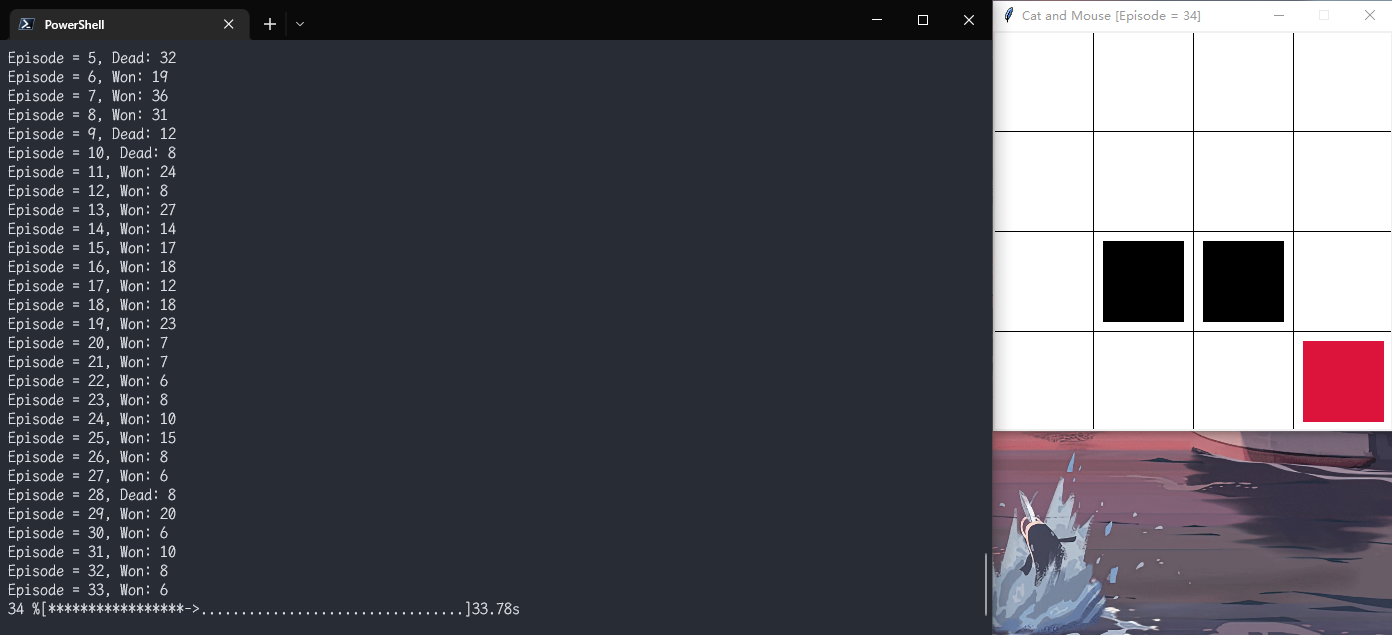
\includegraphics[width=.8\textwidth]{images/1.png}
    \caption{老鼠固定}
    \label{fig:1}
\end{figure}

\subsection{老鼠游走}

老鼠游走时,强化学习如图\ref{fig:2}所示。此时,由于老鼠在随机游走,学习速度编码,在 6、70 次训练之后,猫才能够比较稳定地抓住老鼠。

\begin{figure}[H]
    \centering
    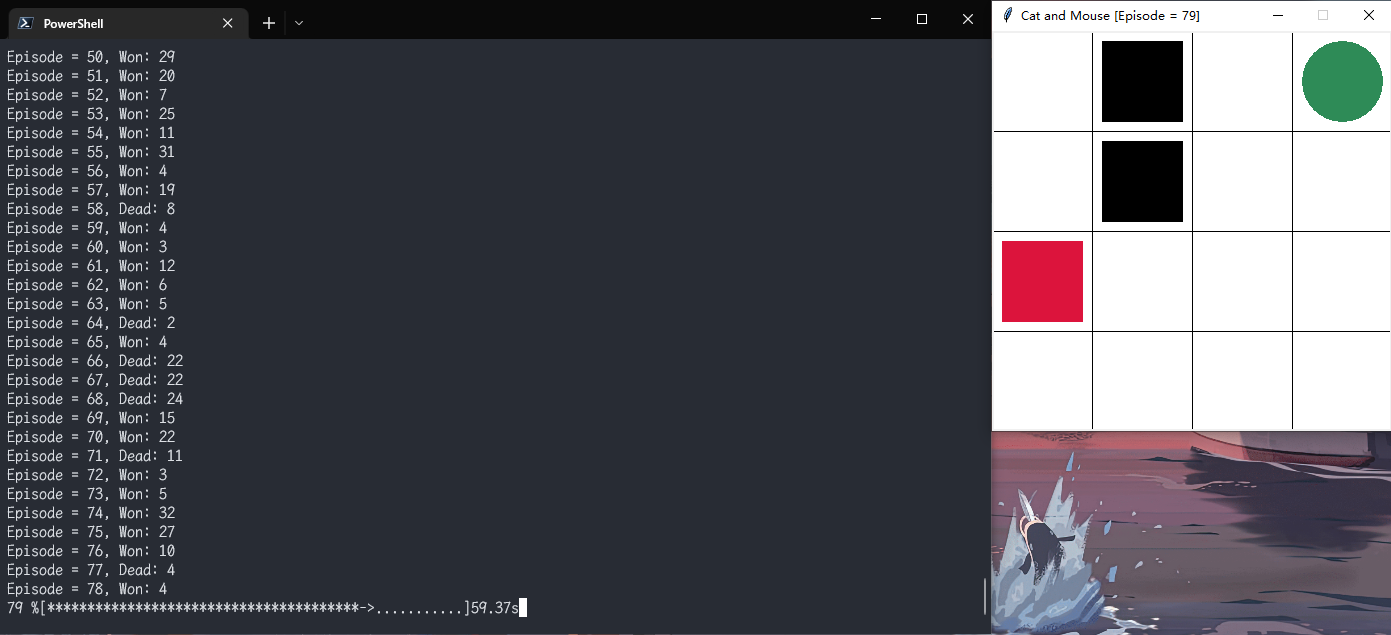
\includegraphics[width=.8\textwidth]{images/2.png}
    \caption{老鼠游走}
    \label{fig:2}
\end{figure}

\subsection{增加格子}

增加格子到 $50\times 50$,同时障碍为 40 时,强化学习如图\ref{fig:3}所示。此时,由于棋盘过大,需要更多的迭代次数才能够更新 Q 表,时间过长,但是整体的逻辑是一样的。

\begin{figure}[H]
    \centering
    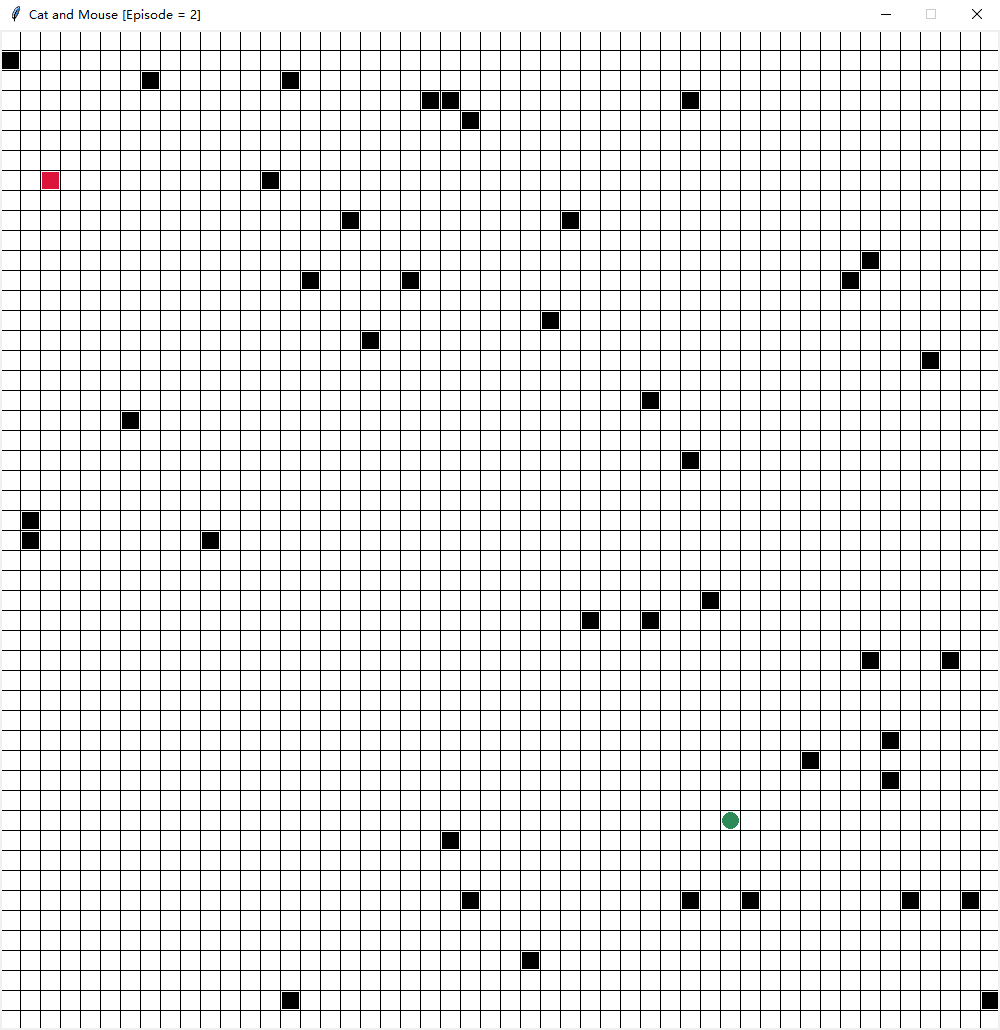
\includegraphics[width=.8\textwidth]{images/3.png}
    \caption{增加格子}
    \label{fig:3}
\end{figure}

\section{总结}

通过这次强化学习的练习,我熟悉了Q Learning 学习和更新的策略,同时体验了强化学习的趣味所在,收获颇大。最后感谢老师和助教的辛勤付出!

\end{document}
